\documentclass[11pt,compress,t,notes=noshow, aspectratio=169, xcolor=table]{beamer}

% Can only be executed locally, as the 'lecture_iml' submodule is accessed (which is not included in Overleaf). 
% Before executing this script, please ensure that the latest PDF files are available in the 'slides-pdf' folder in 'lecture_iml'.

\usepackage{../../style/lmu-lecture}
\usepackage{pdfpages}
% Defines macros and environments
% This file is included in slides and exercises

% Rarely used fontstyle for R packages, used only in 
% - forests/slides-forests-benchmark.tex
% - exercises/single-exercises/methods_l_1.Rnw
% - slides/cart/attic/slides_extra_trees.Rnw
\newcommand{\pkg}[1]{{\fontseries{b}\selectfont #1}}

% Spacing helpers, used often (mostly in exercises for \dlz)
\newcommand{\lz}{\vspace{0.5cm}} % vertical space (used often in slides)
\newcommand{\dlz}{\vspace{1cm}}  % double vertical space (used often in exercises, never in slides)
\newcommand{\oneliner}[1] % Oneliner for important statements, used e.g. in iml, algods
{\begin{block}{}\begin{center}\begin{Large}#1\end{Large}\end{center}\end{block}}

% Don't know if this is used or needed, remove?
% textcolor that works in mathmode
% https://tex.stackexchange.com/a/261480
% Used e.g. in forests/slides-forests-bagging.tex
% [...] \textcolor{blue}{\tfrac{1}{M}\sum^M_{m} [...]
% \makeatletter
% \renewcommand*{\@textcolor}[3]{%
%   \protect\leavevmode
%   \begingroup
%     \color#1{#2}#3%
%   \endgroup
% }
% \makeatother



\title{Interpretable Machine Learning}
% \author{LMU}
%\institute{\href{https://compstat-lmu.github.io/lecture_iml/}{compstat-lmu.github.io/lecture\_iml}}
\date{}

\begin{document}


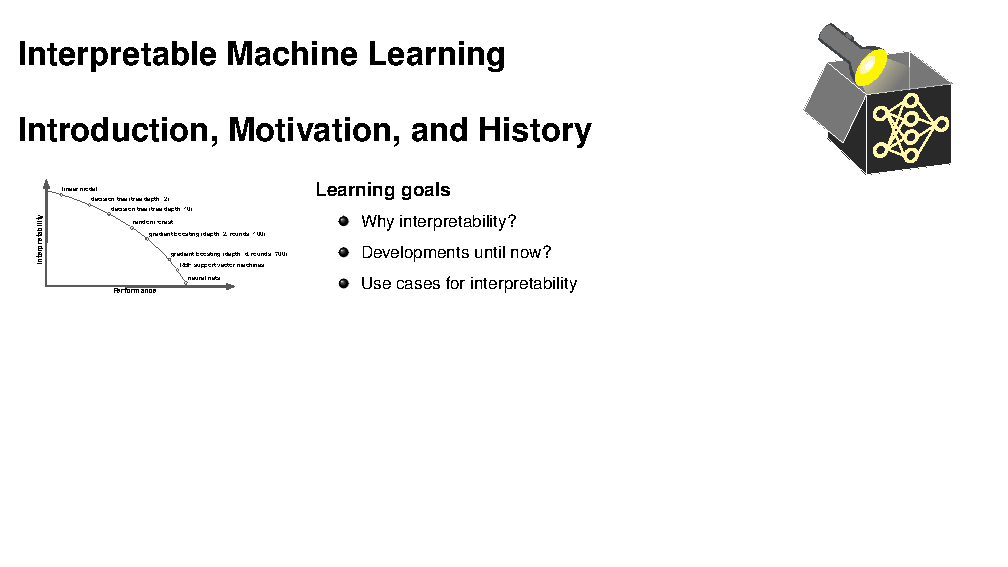
\includepdf[pages={1-6}]{../../lecture_iml/slides-pdf/slides01-intro-motivation.pdf}
% 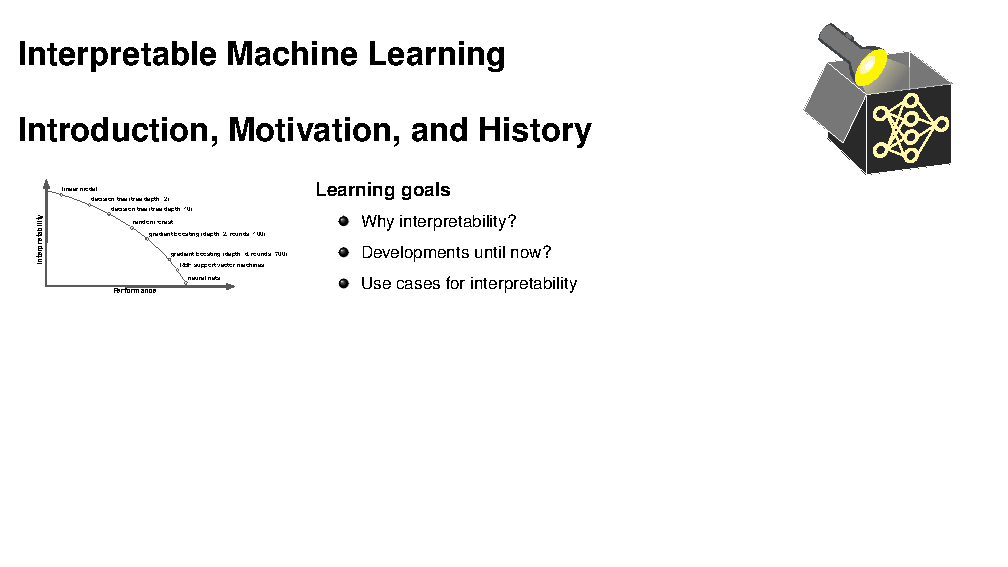
\includepdf[pages={1}]{../../lecture_iml/slides-pdf/slides01-intro-motivation.pdf}

% 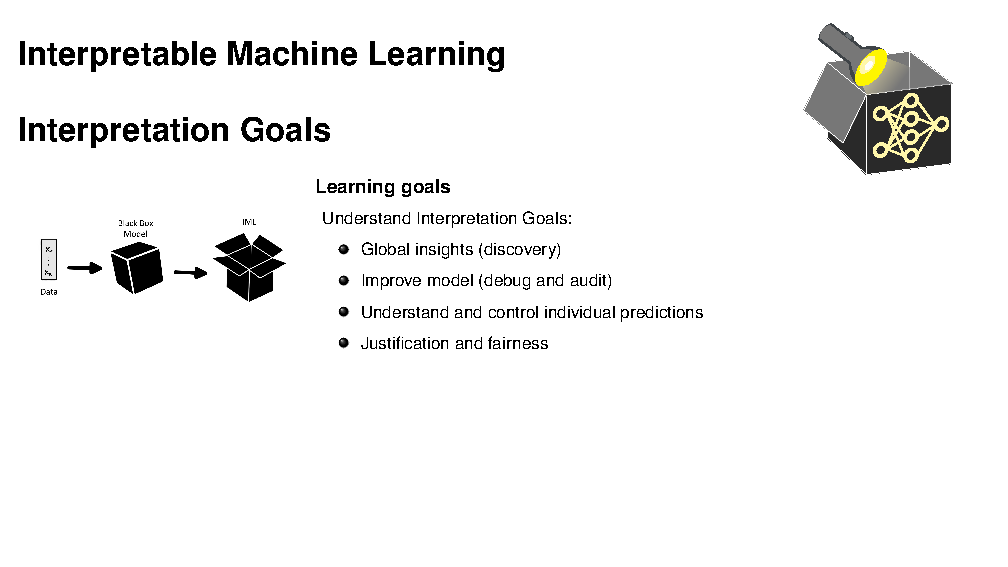
\includepdf[pages=-]{../../lecture_iml/slides-pdf/slides02-intro-goals.pdf}

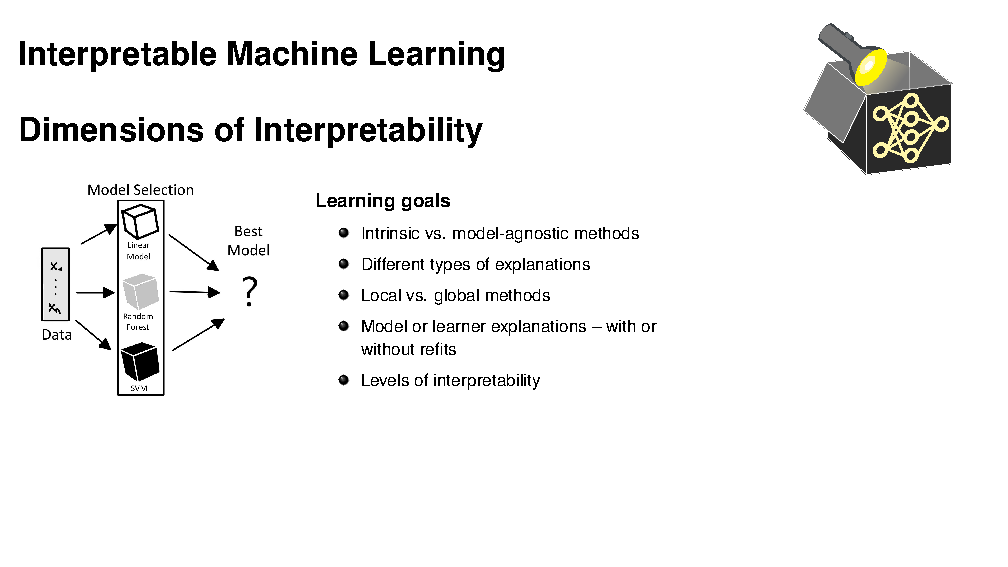
\includepdf[pages={1-13}]{../../lecture_iml/slides-pdf/slides03-intro-dimensions.pdf}

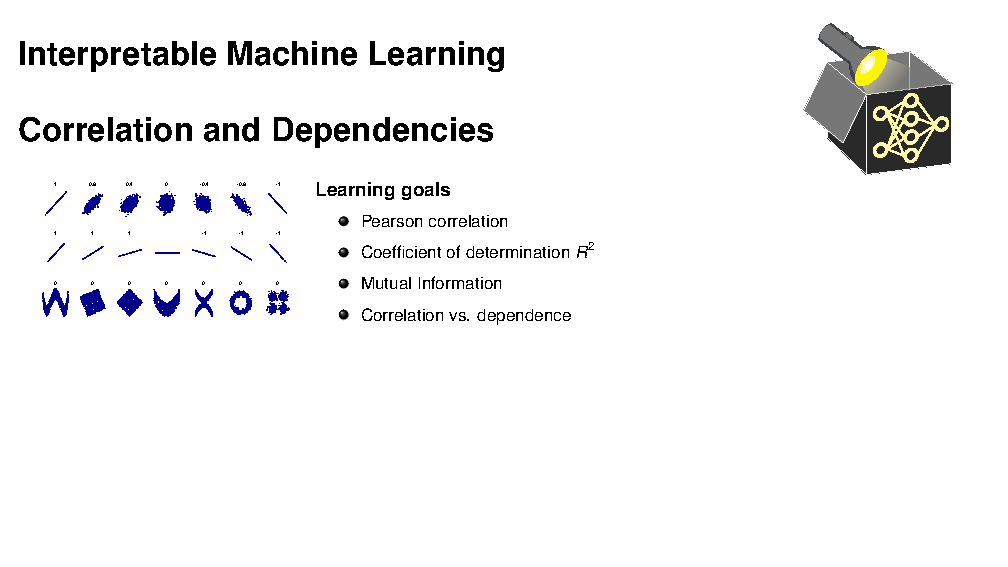
\includepdf[pages={1,10-12,14-20}]{../../lecture_iml/slides-pdf/slides04-intro-correlation.pdf}

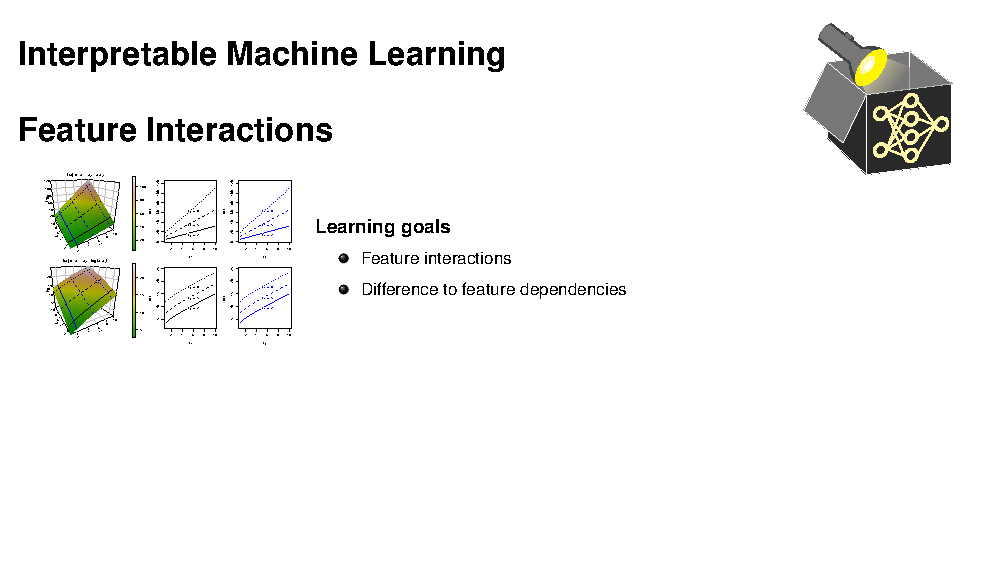
\includepdf[pages=-]{../../lecture_iml/slides-pdf/slides05-intro-interaction.pdf}


\end{document}